\documentclass[12pt]{article}

\usepackage{amsmath,amssymb}
\usepackage{graphicx}
\usepackage{booktabs}
\usepackage{multirow}
\usepackage{float}
\usepackage{algorithm}
\usepackage{algpseudocode}
\usepackage{hyperref}
\usepackage[margin=1in]{geometry}
\usepackage{xcolor}
\usepackage{caption}

\hypersetup{
  colorlinks=true,
  linkcolor=blue,
  citecolor=blue,
  urlcolor=blue,
}

\title{Enhancing the MADDPG Algorithm via Pre-Trained Action Inference\\
       in Competitive Multi-Agent Environments}

\author{Shaash Sivakumar, Marc Walden, Jason Liu, Ryan Liu, Hamza Khan\\
\small UCLA Mathematics Department}

\date{May 2025}

\begin{document}

\maketitle

\begin{abstract}
We investigate multi-agent deep reinforcement learning in competitive environments and
propose an enhancement to the Multi-Agent Deep Deterministic Policy Gradient (MADDPG)
algorithm through a novel \emph{Pre-Trained Action Inference} (PTAI) mechanism. PTAI
pre-trains a dedicated neural network offline---using only randomly generated interaction
data---to predict each agent's previous joint action vector from temporally stacked
observations. These inferred actions are then concatenated to each agent's local
observation before it enters the actor network, providing a richer behavioural context
for policy learning without introducing any new online gradient interactions. We evaluate
both baseline MADDPG and MADDPG+PTAI on four competitive Mixed Physical Environments
(MPE) from the PettingZoo library across 3--4 independent random seeds each. PTAI
yields consistent, large improvements across all four environments: $+104\%$ in Physical
Deception (\texttt{simple\_adversary\_v3}), $+83\%$ in Cooperative Push
(\texttt{simple\_push\_v3}), $+157\%$ in Keep-Away
(\texttt{simple\_world\_comm\_v3}), and $+437\%$ in Predator-Prey
(\texttt{simple\_tag\_v3}). Our results suggest that conditioning each agent's policy on
inferred peer behaviour from a frozen pre-trained module is a simple and broadly effective
strategy for improving coordination and counter-strategy in multi-agent systems.
\end{abstract}

\tableofcontents
\newpage

% =============================================================================
\section{Introduction}
% =============================================================================

Multi-agent reinforcement learning (MARL) addresses settings in which multiple autonomous
agents must simultaneously learn effective policies while interacting within a shared
environment~\cite{busoniu2008comprehensive}. Such settings arise naturally in robotics,
autonomous vehicles, strategic game playing, and network resource allocation, among other
domains. A defining challenge in MARL is \emph{non-stationarity}: from any single agent's
perspective, the environment appears to change over time because the policies of all other
agents are simultaneously evolving. This violates the Markov property that underpins most
single-agent RL convergence results, and can cause independent learners to oscillate or
diverge~\cite{tan1993multi}.

Actor-critic algorithms partially address non-stationarity by combining a low-variance
critic baseline with a policy-gradient actor update~\cite{mnih2016asynchronous}. The
Multi-Agent Deep Deterministic Policy Gradient (MADDPG) algorithm~\cite{lowe2017multi}
goes further by adopting a \emph{centralised training, decentralised execution} (CTDE)
paradigm: each agent maintains a centralised critic that observes the full joint
observation-action tuple during training, while each actor relies only on the agent's
local observation at execution time. This formulation substantially stabilises learning
because the centralised critic can directly account for the actions of all agents.

Even so, the MADDPG critic uses only \emph{current}-step joint information. In competitive
settings where agents must anticipate and react to opponents' strategies, knowledge of
what each agent did in the previous step carries important information about short-term
intent. Yet this temporal context is absent from both the actor's input (which sees only
the current local observation) and the critic's input (which sees current joint
observations and actions).

We address this gap with \emph{Pre-Trained Action Inference} (PTAI). A dedicated AI\_Net
module is trained offline---before any MADDPG gradient updates---on random interaction
data to predict the previous joint action vector from a pair of consecutive local
observations. Once pre-trained, the AI\_Net is frozen and used at every decision step to
supply each agent's actor with an estimate of the previous joint action, concatenated to
its current observation. Because the AI\_Net is stationary and requires no online updates,
it adds no training instability. At the same time, it endows each actor with temporal
context that would otherwise be inaccessible.

\paragraph{Contributions.}
\begin{enumerate}
\item We describe a modular PTAI architecture that exploits the structural separability of
      MPE observations to infer previous joint actions efficiently via Directional Social
      and Self-Awareness modules.
\item We extend the evaluation of PTAI from a single environment (Predator-Prey) to four
      competitive MPE environments, with 3--4 independent seeds per condition.
\item We report quantitative, seed-averaged results with standard deviations, demonstrating
      that PTAI consistently and substantially outperforms baseline MADDPG across all
      tested environments.
\end{enumerate}

For the initial implementation of standard MADDPG we adapted an open-source codebase~\cite{git123hub2021}, then rebuilt and extended it with the PTAI mechanism described here.

% =============================================================================
\section{Background}
% =============================================================================

\subsection{Reinforcement Learning Framework}

In a standard reinforcement learning (RL) setting, an agent interacts with an environment
$\mathcal{E}$ over discrete time steps $t = 0, 1, 2, \ldots$~\cite{sutton2018reinforcement}.
At each step, the agent observes $o^i_t \in \mathcal{O}$, selects an action
$a^i_t \in \mathcal{A}$, and receives a scalar reward $r^i_{t+1} \in \mathbb{R}$.
The agent's goal is to learn a policy $\pi_{\theta_i}(a^i \mid o^i)$, parameterised by
$\theta_i$, that maximises the expected discounted return:
\begin{equation}
J(\theta_i) \;=\; \mathbb{E}\!\left[\sum_{t=0}^{\infty} \gamma^t r^i_{t+1}\right],
\label{eq:return}
\end{equation}
where $\gamma \in [0, 1)$ is the discount factor. The most common approach to optimising
Equation~\eqref{eq:return} is General Policy Iteration (GPI), which alternates between
policy evaluation (estimating the current value function) and policy improvement (refining
the policy to increase expected value).

\subsection{Deep Q-Learning and Multi-Agent Extensions}

Mnih et al.~\cite{mnih2015human} introduced the Deep Q-Network (DQN), which approximates
the action-value function $Q(s, a)$ with a deep neural network and minimises the Bellman
error
\begin{equation}
\mathcal{L}(\phi) \;=\; \mathbb{E}_{(s,a,r,s') \sim \mathcal{D}}
  \left[\!\left(r + \gamma \max_{a'} Q_{\phi^-}(s', a') - Q_\phi(s, a)\right)^{\!2}\right],
\label{eq:dqn}
\end{equation}
where $\mathcal{D}$ is an experience replay buffer. DQN excels in single-agent settings
but becomes unstable in multi-agent environments because each agent's policy updates
effectively change the environment dynamics for all others.

Tan~\cite{tan1993multi} applied independent Q-learning to multi-agent problems, but the
resulting non-stationarity is well documented. Addressing this motivated the centralised
critic approach of MADDPG.

\subsection{Policy-Gradient Methods and MADDPG}

Policy-gradient methods directly optimise $J(\theta)$ by gradient ascent:
$\theta \leftarrow \theta + \alpha \nabla_\theta J(\theta)$.
The Policy Gradient theorem~\cite{sutton1999policy} gives:
\begin{equation}
\nabla_\theta J(\theta) \;=\; \mathbb{E}\!\left[\nabla_\theta \log \pi_\theta(a \mid o)\; Q^\pi(o, a)\right].
\end{equation}

MADDPG~\cite{lowe2017multi} extends deterministic policy gradients~\cite{silver2014deterministic}
to the multi-agent setting by giving each agent $i$ a decentralised actor $\mu_{\theta_i}(o_i)$
and a centralised critic $Q_{\phi_i}(x, a_{1:N})$, where $x$ is the global joint observation and
$a_{1:N}$ the joint action. Each critic is trained to minimise
\begin{equation}
\mathcal{L}(\phi_i) \;=\; \frac{1}{S}\sum_j
  \bigl(y^j - Q_{\phi_i}(x^j, a^j_1, \ldots, a^j_N)\bigr)^2, \quad
y^j = r^j_i + \gamma Q_{\phi_i'}\!\bigl(x'^j, a'^j_1, \ldots, a'^j_N\bigr),
\label{eq:critic_loss}
\end{equation}
and each actor is updated by the sampled deterministic policy gradient:
\begin{equation}
\nabla_{\theta_i} J \;\approx\; \frac{1}{S}\sum_j
  \nabla_{\theta_i} \mu_i(o^j_i)\;
  \nabla_{a_i} Q_{\phi_i}(x^j, a^j_1, \ldots, a_i, \ldots, a^j_N)
  \Big|_{a_i = \mu_i(o^j_i)}.
\label{eq:actor_grad}
\end{equation}
During execution each agent acts based only on its local observation $o_i$, preserving
scalability and decentralisation. Target networks (soft-updated at rate $\tau$) and a
shared experience replay buffer ensure stable training. The full algorithm is given as
Algorithm~\ref{alg:maddpg} in the appendix.

% =============================================================================
\section{Method: Pre-Trained Action Inference (PTAI)}
% =============================================================================

\subsection{Motivation}

In competitive MARL, the quality of an agent's decision depends not only on its current
observation but also on what other agents have just done. Two otherwise identical states
can call for very different actions depending on whether, e.g., an opponent just moved
aggressively or retreated. Standard MADDPG actors have no direct access to this temporal
context: the actor sees only the current observation $o^t_i$, and the previous joint action
$(a^{t-1}_1, \ldots, a^{t-1}_N)$ is not stored separately in the standard replay buffer.

PTAI provides this missing temporal signal by inferring the previous joint action from
the change in observations---without requiring communication between agents or access to
opponents' policies.

\subsection{AI\_Net Architecture}

Let $N$ be the number of agents. Each agent $i$ maintains its own instance of an
\emph{AI\_Net} that maps
\begin{equation}
\widehat{\mathbf{a}}_i \;=\; \text{AI\_Net}(o^t_i, o^{t-1}_i),
\label{eq:ainet}
\end{equation}
where $o^t_i, o^{t-1}_i \in \mathbb{R}^{d_i}$ are the current and previous observations
of agent $i$, and $\widehat{\mathbf{a}}_i \in \mathbb{R}^{\sum_k |\mathcal{A}_k|}$ is an
estimate of the full previous joint action vector
$\text{concat}(\text{onehot}(a^{t-1}_1), \ldots, \text{onehot}(a^{t-1}_N))$.

The key structural insight is that many MPE observation vectors are \emph{separable}:
different contiguous segments correspond to features of different agent types. This
allows AI\_Net to decompose the prediction task into smaller specialised modules rather
than one monolithic network (which would scale as $O(N^2)$ in parameters).

\paragraph{Directional Social Awareness Modules.}
For each ordered pair (observer type $p$, observed type $q$), a Social Awareness module
takes as input the features in $o^t_i$ and $o^{t-1}_i$ that pertain to an agent of type
$q$, together with the self/global features of observer $i$, and outputs a prediction of
that agent's previous action:
\begin{equation}
\widehat{a}_{i,k} \;=\; \mathbf{Social}_\theta(o_{i,k}, o_{i,g},
  o^-_{i,k}, o^-_{i,g}, \Delta o_{i,k}, \Delta o_{i,g}),
\end{equation}
where $o_{i,k}$ are the features in agent $i$'s observation relating to agent $k$,
$o_{i,g}$ are global/self features, superscript $^-$ denotes the previous-step value,
and $\Delta = o^t - o^{t-1}$ is the temporal difference.

\paragraph{Directional Self-Awareness Module.}
A Self-Awareness module predicts the agent's own previous action from its self/global
features and their temporal difference:
\begin{equation}
\widehat{a}_{i,i} \;=\; \mathbf{Self}_\theta(o_{i,i}, o_{i,g},
  o^-_{i,i}, o^-_{i,g}, \Delta o_{i,i}, \Delta o_{i,g}).
\end{equation}

The complete joint action estimate is
$\widehat{\mathbf{a}}_i = (\widehat{a}_{i,1}, \ldots, \widehat{a}_{i,N})$,
where each component is the output of the appropriate Social or Self module routed
by AI\_Net according to agent types.

A diagram of the full AI\_Net architecture is shown in Figure~\ref{fig:ainet_diagram}.

\begin{figure}[H]
\centering
\includegraphics[width=0.80\textwidth]{ainet_diagram.png}
\caption{AI\_Net architecture for separable observations. Each pair of temporally stacked
observation parameters undergoes an arithmetic difference operation, creating temporal
difference features. Features are grouped by the agent they pertain to and routed to the
corresponding Directional Social Awareness Module. Self/global features are routed to the
Directional Self-Awareness Module to predict the observer's own previous action.}
\label{fig:ainet_diagram}
\end{figure}

\subsection{Pre-Training Procedure}

AI\_Net is pre-trained offline on $P = 200$ episodes of random interaction (all agents
sampling uniformly from their action spaces) prior to any MADDPG training. At each step,
all awareness modules are updated by minimising the mean-squared error between predicted
and true one-hot actions (Algorithm~\ref{alg:ptai} in the appendix). A stochastic
sampling gate randomly drops a fraction of training pairs to improve generalisation.

After pre-training, the weights of all modules are \emph{frozen}. Because the AI\_Net is
completely stationary, it introduces no additional optimisation interaction with the MADDPG
training loop and imposes no extra computational cost per gradient step.

\subsection{Integration with MADDPG}

At each decision step $t \geq 2$, for each agent $i$, the frozen AI\_Net is queried:
\begin{equation}
\widehat{\mathbf{a}}^t_i \;=\; \text{AI\_Net}(o^t_i, o^{t-1}_i).
\end{equation}
The actor input is extended to:
\begin{equation}
\mu_{\theta_i}\!\left([o^t_i \;\|\; \widehat{\mathbf{a}}^t_i]\right),
\label{eq:actor_ptai}
\end{equation}
where $\|$ denotes concatenation. At the first step of each episode (no previous
observation available), $\widehat{\mathbf{a}}^t_i$ is replaced by a zero vector of the
same dimension. The centralised critic retains its standard input
$Q_{\phi_i}(x^t, a^t_1, \ldots, a^t_N)$. The complete MADDPG+PTAI training loop is
given as Algorithm~\ref{alg:maddpg_ptai} in the appendix.

\paragraph{Interpretation.}
By conditioning the actor on inferred peer actions, each agent's policy can explicitly
account for the recent joint behaviour of all agents, even without direct communication.
In competitive settings this enables agents to develop reactive strategies (e.g.\
predators coordinating their approach based on each other's last move) that would not be
accessible from the current observation alone. Because the AI\_Net is pre-trained on
random actions---not the current MADDPG policy---it provides a general-purpose,
policy-agnostic temporal signal that remains useful throughout training.

% =============================================================================
\section{Environments}
% =============================================================================

We evaluate on four competitive MPE environments from the PettingZoo library~\cite{terry2021pettingzoo}, all featuring a team of ``good'' agents (prefixed \texttt{agent\_}) and a team of adversaries (prefixed \texttt{adversary\_}) that learn concurrently via standard MADDPG co-training. Table~\ref{tab:envs} summarises the key properties.

\begin{table}[H]
\centering
\caption{Competitive MPE environments used in this study.}
\label{tab:envs}
\begin{tabular}{lcccp{4.2cm}}
\toprule
Environment & Agents & Adversaries & Metric & Description \\
\midrule
\texttt{simple\_adversary\_v3}   & 2 & 1 & Agent reward          & Adversary blends among landmarks to reach its target while good agents try to identify it \\
\texttt{simple\_push\_v3}        & 1 & 1 & Agent win rate        & Agent navigates to its goal; adversary tries to block it \\
\texttt{simple\_tag\_v3}         & 1 & 3 & Catches per episode   & Three predators cooperate to tag a faster-moving prey \\
\texttt{simple\_world\_comm\_v3} & 2 & 4 & Adversary frames at goal & Adversaries try to reach the good agents' secret target \\
\bottomrule
\end{tabular}
\end{table}

\paragraph{Physical Deception (\texttt{simple\_adversary\_v3}).}
Three landmarks are placed in the arena. One landmark is the adversary's secret target.
The adversary blends in among all landmarks to reach its goal without being identified.
The two good agents want to cover all landmarks and determine which the adversary is
heading toward. We report the episode reward of the good agent team, averaged over the
last 1\,000 of 30\,000 training episodes. Higher values indicate better good-agent
performance; the adversary is treated as part of the (co-training) environment from the
agents' perspective.

\paragraph{Cooperative Push (\texttt{simple\_push\_v3}).}
A single good agent must navigate to its goal landmark while a single adversary attempts
to physically push it away and simultaneously reach its own goal. We measure the
\emph{agent win rate}: the fraction of episodes in which the good agent occupies its
goal landmark at episode termination.

\paragraph{Predator-Prey (\texttt{simple\_tag\_v3}).}
Three predators (adversary team) cooperate to catch a prey (agent team). The prey moves
faster than any single predator, requiring the predators to coordinate their pursuit.
We measure the mean number of \emph{catches per episode}, where a catch occurs whenever
a predator is within tagging distance of the prey. PTAI is particularly relevant here
because the predators must anticipate each other's movements to avoid redundant pursuit
directions and successfully encircle the prey.

\paragraph{Keep-Away (\texttt{simple\_world\_comm\_v3}).}
Four adversaries attempt to reach the true goal landmark that only the good-agent speaker
knows. The good agents have a shared communication channel but cannot prevent adversaries
from receiving it. We measure \emph{adversary frames at goal}: the total number of
time steps per episode in which at least one adversary occupies the goal landmark.
Higher scores represent better adversary performance; PTAI applied to the adversary team
benefits from their team-level coordination in locating and converging on the goal.

% =============================================================================
\section{Experiments}
% =============================================================================

\subsection{Training Setup}

All experiments use a common set of hyperparameters (Table~\ref{tab:hparams}) applied to
both baseline MADDPG and MADDPG+PTAI.

\begin{table}[H]
\centering
\caption{Training hyperparameters (shared across all experiments).}
\label{tab:hparams}
\begin{tabular}{lc}
\toprule
Hyperparameter & Value \\
\midrule
Training episodes     & 30\,000 \\
Warmup steps          & 50\,000 \\
Replay buffer capacity & 1\,000\,000 \\
Batch size            & 1\,024 \\
Discount factor $\gamma$ & 0.95 \\
Soft-update rate $\tau$ & 0.02 \\
Actor/Critic learning rate & 0.01 \\
Checkpoint interval   & 10\,000 episodes \\
\bottomrule
\end{tabular}
\end{table}

\paragraph{Network architecture.}
All actor networks are two-hidden-layer MLPs (observation $\to$ 64 $\to$ 64 $\to$ action),
initialised with Xavier-uniform weights and $0.01$ bias constants.
Discrete actions are produced via Gumbel-Softmax~\cite{jang2017categorical} during training
(enabling differentiable action samples) and argmax at evaluation time.
Critic networks share the same MLP architecture but take the full joint observation-action
vector as input.
All gradients are clipped at a global norm of $0.5$, and actor losses include a small
logit regulariser ($10^{-3} \times \overline{\|\text{logits}\|^2}$) to prevent
policy collapse.

For MADDPG+PTAI, the actor input dimension is expanded by
$\sum_k |\mathcal{A}_k|$ to accommodate the inferred previous joint action vector
$\widehat{\mathbf{a}}_i \in \mathbb{R}^{\sum_k |\mathcal{A}_k|}$.

\paragraph{PTAI pre-training.}
The AI\_Net is pre-trained for 200 episodes of uniformly random play (all agents sample
uniformly from their action space) before MADDPG training begins. If a pre-trained
\texttt{AI\_Net.pt} checkpoint already exists in the project root, it is loaded without
re-training. The Social and Self-Awareness modules are two-layer MLPs with 64 hidden
units, trained with Adam at learning rate $10^{-3}$.

\subsection{Evaluation Protocol}

For each (environment, algorithm) pair we run $n = 3$--$4$ independent seeds (see
Table~\ref{tab:results} for per-cell $n$). Performance is measured as the mean episode
metric over the \emph{last 1\,000 training episodes} of each run, a window that reflects
converged policy quality while averaging out short-term volatility. We report the
cross-seed mean $\pm$ standard deviation (sample, $n-1$ denominator).

The metrics reported are:
\begin{itemize}
  \item \textbf{Agent reward} (\texttt{simple\_adversary\_v3}): Episode reward of the
        good agent team (higher = better for agents).
  \item \textbf{Agent win rate} (\texttt{simple\_push\_v3}): Fraction of episodes in
        which the good agent is at its goal at episode end (higher = better for agents).
  \item \textbf{Catches per episode} (\texttt{simple\_tag\_v3}): Mean number of
        predator-prey contact events per episode (higher = better for predators).
  \item \textbf{Adversary frames at goal} (\texttt{simple\_world\_comm\_v3}): Mean
        number of time steps per episode during which at least one adversary occupies the
        goal landmark (higher = better for adversaries).
\end{itemize}

For \texttt{simple\_tag\_v3} and \texttt{simple\_push\_v3}, the reported metric is
derived from the environment-specific metric tracker rather than raw episode reward.
For \texttt{simple\_adversary\_v3}, metric tracking was unavailable for the earliest seed
of the baseline (which predates the metric system); we use the raw episode reward directly
for all four baseline seeds, which is consistent across runs.

% =============================================================================
\section{Results}
% =============================================================================

\subsection{Quantitative Summary}

Table~\ref{tab:results} reports the main results. MADDPG+PTAI outperforms baseline MADDPG
on all four environments, with improvements ranging from $+83\%$ to $+437\%$.

\begin{table}[H]
\centering
\caption{Final-policy performance: mean $\pm$ std over the last 1\,000 training episodes,
averaged across $n$ independent seeds. $\Delta$ is the relative improvement of PTAI over
the baseline. All differences favour PTAI.}
\label{tab:results}
\begin{tabular}{lllllll}
\toprule
Environment & Metric & MADDPG ($n$) & MADDPG+PTAI ($n$) & $\Delta$ \\
\midrule
\texttt{simple\_adversary\_v3}
  & Agent reward
  & $9.91 \pm 0.40$ (4)
  & $20.22 \pm 2.82$ (4)
  & $+104\%$ \\
\texttt{simple\_push\_v3}
  & Agent win rate
  & $0.18 \pm 0.08$ (3)
  & $0.33 \pm 0.03$ (4)
  & $+83\%$ \\
\texttt{simple\_tag\_v3}
  & Catches / ep.
  & $0.62 \pm 0.08$ (3)
  & $3.31 \pm 1.59$ (4)
  & $+437\%$ \\
\texttt{simple\_world\_comm\_v3}
  & Adv.\ frames at goal
  & $10.42 \pm 1.72$ (3)
  & $26.78 \pm 2.60$ (4)
  & $+157\%$ \\
\bottomrule
\end{tabular}
\end{table}

\paragraph{Physical Deception.}
Both algorithms achieve moderate positive agent rewards, but PTAI roughly doubles the
baseline's performance ($9.91 \to 20.22$). The good agents benefit from knowing where
the adversary was one step ago, allowing them to better predict which landmark the
adversary is converging on. The larger standard deviation for PTAI ($\pm 2.82$ vs
$\pm 0.40$) suggests that policy quality is more seed-sensitive---some seeds may discover
particularly effective deception-reading strategies that others do not.

\paragraph{Cooperative Push.}
Agent win rates improve from $0.18$ to $0.33$ ($+83\%$). The improvement is also
accompanied by lower variance ($\pm 0.08 \to \pm 0.03$), indicating that PTAI not only
increases performance but also makes it more reproducible. Even knowing only the
adversary's inferred previous action, the agent can better anticipate push directions and
adjust its approach to the goal.

\paragraph{Predator-Prey.}
The most dramatic improvement occurs here: catches per episode rise from $0.62$ to $3.31$,
a $437\%$ increase. This result reflects the high value of temporal coordination
information in a pursuit task. The three predators must spread out and synchronise their
movements to corner the faster prey; without PTAI, each predator acts independently and
often converges on the same direction, making encirclement rare. With PTAI, each predator
can infer where its teammates moved last and adjust to complement their pursuit angles.
The high standard deviation for PTAI ($\pm 1.59$) reflects genuine multi-modality in the
discovered strategies: some seeds discover highly efficient encirclement patterns (up to
$5.44$ catches per episode), while others converge on less effective cooperative behaviours.

\paragraph{Keep-Away.}
Adversary frames at goal improve from $10.42$ to $26.78$ ($+157\%$). The four adversaries
benefit from knowing each other's previous positions relative to the goal, allowing them
to fan out rather than cluster. PTAI produces a tighter cross-seed distribution for both
baseline and PTAI ($\pm 1.72$ and $\pm 2.60$ respectively), consistent with the relatively
deterministic structure of the environment.

\subsection{Training Convergence}

Figure~\ref{fig:convergence} shows smoothed training curves (500-episode running average)
for both algorithms across all four environments. PTAI consistently reaches higher
performance levels and in most environments does so more stably than the baseline.

\begin{figure}[H]
\centering
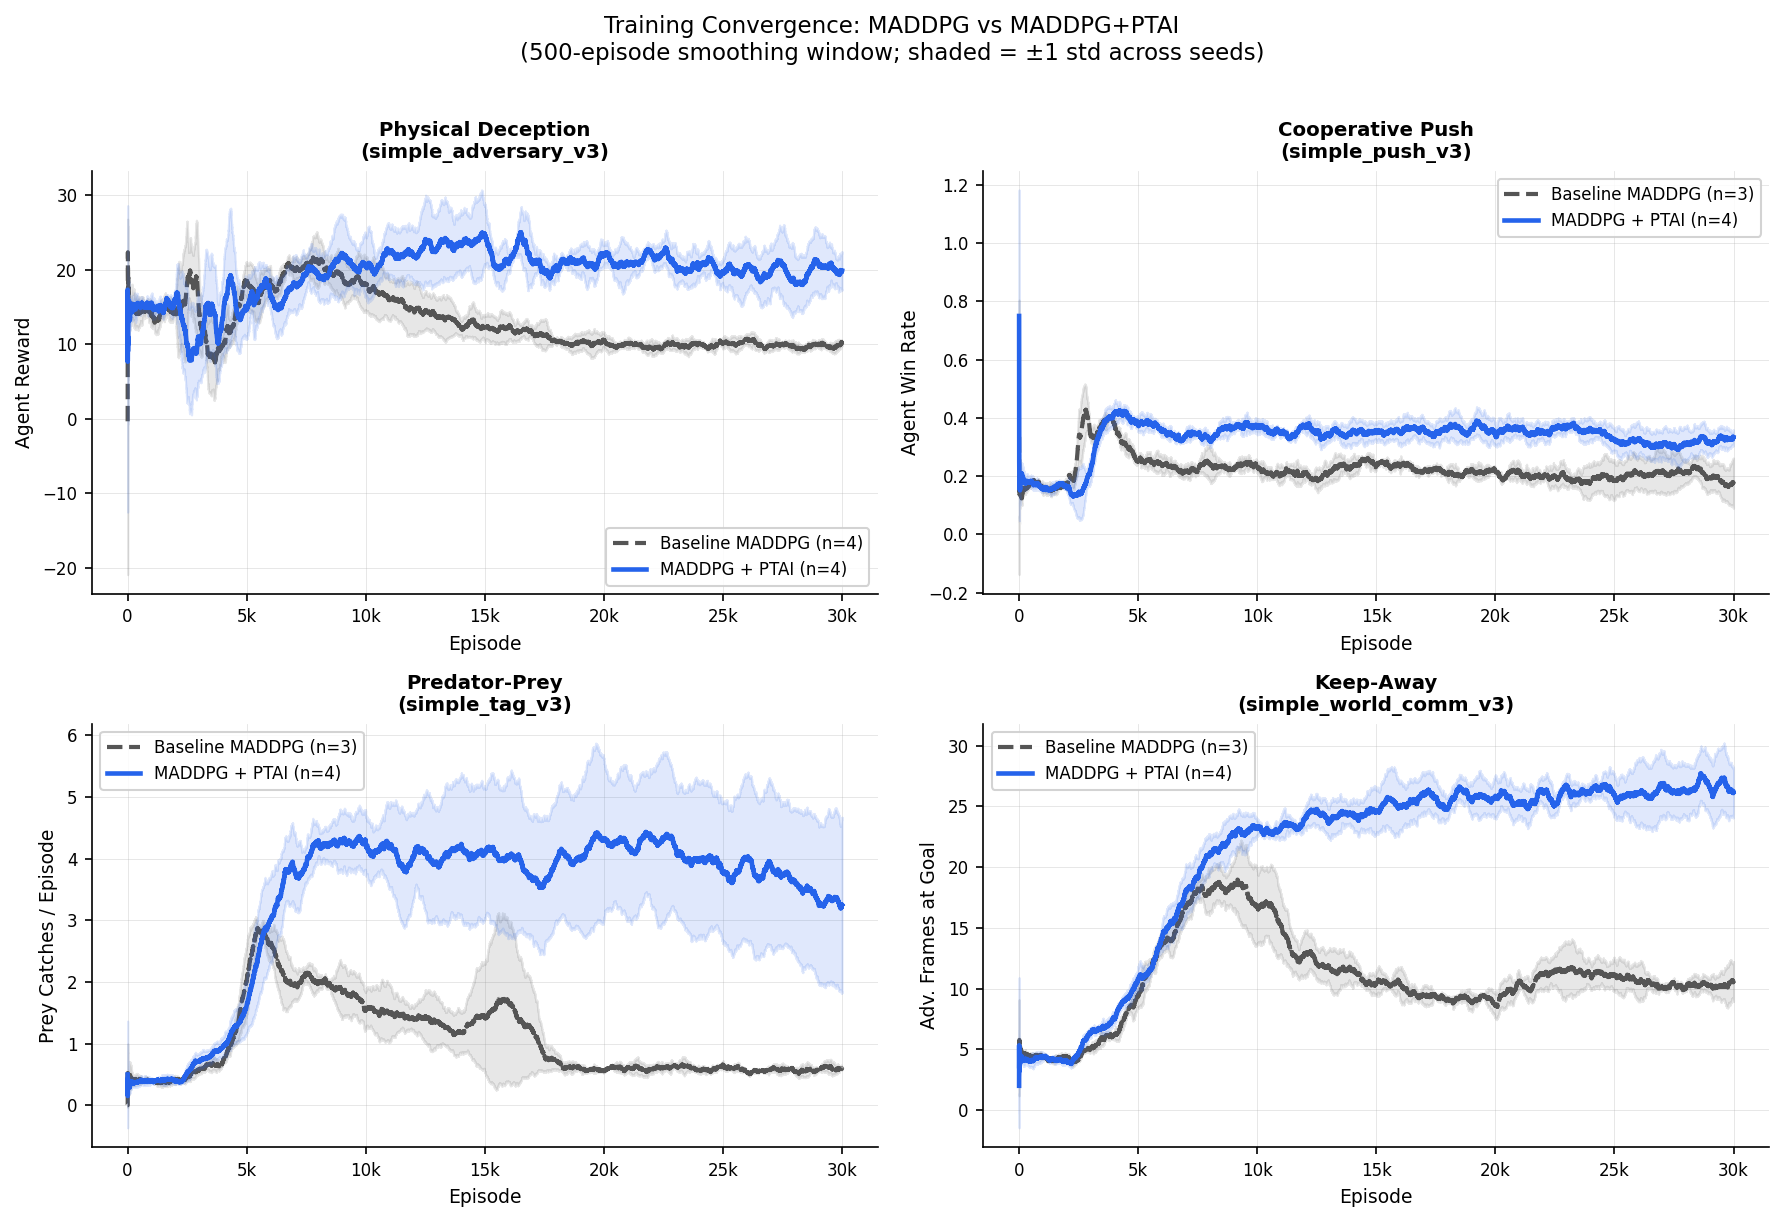
\includegraphics[width=\linewidth]{results/paper_convergence.png}
\caption{Training convergence across four competitive MPE environments. Lines show
the per-episode metric smoothed over a 500-episode window; shaded bands indicate $\pm 1$
standard deviation across seeds. MADDPG+PTAI (blue, solid) consistently outperforms
baseline MADDPG (grey, dashed) across all environments.}
\label{fig:convergence}
\end{figure}

In \texttt{simple\_adversary\_v3} and \texttt{simple\_push\_v3}, PTAI reaches its
advantage early in training and maintains it throughout, suggesting that the inferred
previous-action signal is useful from the start of learning. In \texttt{simple\_tag\_v3},
both algorithms begin near zero catches and diverge markedly after approximately 10\,000
episodes, with PTAI eventually reaching a much higher plateau. In
\texttt{simple\_world\_comm\_v3}, the gap opens gradually and widens to the end of
training, hinting that PTAI's advantages compound over longer training horizons.

% =============================================================================
\section{Discussion}
% =============================================================================

\paragraph{Why does PTAI help?}
PTAI addresses a structural information deficit in the MADDPG actor: the actor sees only
the current observation, which encodes the effects of the previous joint action but not
the action itself. The current observation can be ambiguous---two different joint actions
can produce similar next states. By providing the actor with the inferred previous joint
action, PTAI resolves some of this ambiguity, allowing the actor to condition its policy
on a richer representation of the recent joint trajectory.

This is conceptually related to providing agents with a form of \emph{implicit
communication}: even though agents do not share a communication channel, each agent can
infer what others did by observing how the world changed, and act accordingly. The PTAI
module makes this inference explicit and structured.

\paragraph{Why pre-training on random data?}
Training AI\_Net on random action data rather than MADDPG policy data has two advantages.
First, random data is trivially available and covers the full action space, which
is important during early training when the MADDPG policy explores widely. Second, a
randomly-pre-trained AI\_Net is stationary throughout MADDPG training, which avoids any
interference between AI\_Net and MADDPG gradient updates. Our results suggest that even
imperfect action inference (the AI\_Net is not perfectly accurate) is sufficient to
provide a useful signal.

\paragraph{Environment structure and the size of gains.}
The largest gain occurs in Predator-Prey, the environment with the strongest multi-agent
coordination requirement. Three predators must coordinate spatially, and knowing a
teammate's last move directly informs whether to cut off or pursue. Smaller but still
substantial gains in Physical Deception and Keep-Away suggest that PTAI is broadly useful
in competitive settings even when the coordination structure is less explicit. The
relatively modest gain in Cooperative Push ($+83\%$ vs $+437\%$) may reflect that the
one-vs-one setting provides less opportunity for leveraging multi-agent temporal context.

\paragraph{Limitations.}
PTAI as described here requires that the observation structure is separable enough to
route features to the correct Directional modules. The sub-assignment mappings are
hand-specified per environment (though this is a one-time cost per environment). The
AI\_Net is pre-trained only on random data; future work could explore co-training or
distillation from the current MADDPG policy to improve action inference accuracy as
training progresses. Finally, the high variance on \texttt{simple\_tag\_v3} for PTAI
suggests that the quality of the discovered coordination strategy is sensitive to
initialisation, which warrants investigation of ensemble or curriculum approaches.

% =============================================================================
\section{Conclusion}
% =============================================================================

We presented PTAI, a pre-trained action inference module that provides each agent's actor
with estimates of all agents' previous actions, derived from temporally stacked
observations by a frozen neural network pre-trained on random interaction data. Integrated
into the MADDPG framework, PTAI consistently and substantially improves final-policy
performance across four competitive MPE environments: $+104\%$, $+83\%$, $+157\%$, and
$+437\%$ over baseline MADDPG. The largest gain is in Predator-Prey, a highly
coordination-dependent environment, supporting the interpretation that PTAI is most
valuable when agents must anticipate and complement each other's movements.

Because the AI\_Net is stationary and frozen during MADDPG training, it introduces no
new optimisation interactions, no additional training instability, and negligible
computational overhead. These properties make PTAI a practical drop-in enhancement for
MADDPG and potentially for other CTDE algorithms.

Future work includes extending PTAI to continuous action spaces, exploring online
refinement of the AI\_Net during MADDPG training, and investigating whether similar
temporal inference benefits carry over to fully cooperative environments such as
\texttt{simple\_spread\_v3}.

% =============================================================================
\section*{Acknowledgments}
% =============================================================================

We would like to express our sincere gratitude to Professor Tao Gao for his invaluable
guidance throughout this project. Our work began with a study of the foundational
principles of reinforcement learning as presented in the textbook by Sutton and
Barto~\cite{sutton2018reinforcement}. Following Professor Gao's recommendation, we
explored various implementations of deep reinforcement learning, drawing on the works
of Yu et al.~\cite{yu2021surprising} and Chen et al.~\cite{chen2016decentralized}, which
led us to the domain of multi-agent reinforcement learning and ultimately to the MADDPG
algorithm of Lowe et al.~\cite{lowe2017multi}, later made available via the PettingZoo
library by the Farama Foundation~\cite{terry2021pettingzoo}. We integrated the MADDPG
algorithm by adapting an existing codebase from Git-123-Hub~\cite{git123hub2021},
modifying it substantially to suit our project. Our code is available at
\url{https://github.com/shaashwathsivakumar/MARL_Proj}.

% =============================================================================
\bibliographystyle{plain}
\begin{thebibliography}{99}

\bibitem{busoniu2008comprehensive}
L.\ Bus\c{o}niu, R.\ Babu\v{s}ka, and B.\ De Schutter.
A comprehensive survey of multi-agent reinforcement learning.
\textit{IEEE Transactions on Systems, Man, and Cybernetics, Part C}, 38(2):156--172, 2008.

\bibitem{chen2016decentralized}
Y.\ F.\ Chen, M.\ Everett, M.\ Liu, and J.\ P.\ How.
Decentralized non-communicating multiagent collision avoidance with deep reinforcement learning, 2016.

\bibitem{git123hub2021}
Git-123-Hub.
\textit{maddpg-pettingzoo-pytorch}.
\url{https://github.com/Git-123-Hub/maddpg-pettingzoo-pytorch}, 2021.
GitHub repository.

\bibitem{jang2017categorical}
E.\ Jang, S.\ Gu, and B.\ Poole.
Categorical reparameterization with Gumbel-Softmax.
In \textit{ICLR}, 2017.

\bibitem{lowe2017multi}
R.\ Lowe, Y.\ Wu, A.\ Tamar, J.\ Harb, P.\ Abbeel, and I.\ Mordatch.
Multi-agent actor-critic for mixed cooperative-competitive environments.
In \textit{NeurIPS}, 2017.

\bibitem{mnih2015human}
V.\ Mnih, K.\ Kavukcuoglu, D.\ Silver, A.\ A.\ Graves, I.\ Antonoglou, D.\ Wierstra,
and M.\ Riedmiller.
Playing Atari with deep reinforcement learning.
In \textit{NeurIPS}, 2013.

\bibitem{mnih2016asynchronous}
V.\ Mnih, A.\ P.\ Badia, M.\ Mirza, A.\ Graves, T.\ Harley, T.\ P.\ Lillicrap,
D.\ Silver, and K.\ Kavukcuoglu.
Asynchronous methods for deep reinforcement learning.
In \textit{ICML}, 2016.

\bibitem{silver2014deterministic}
D.\ Silver, G.\ Lever, N.\ Heess, T.\ Degris, D.\ Wierstra, and M.\ Riedmiller.
Deterministic policy gradient algorithms.
In \textit{ICML}, 2014.

\bibitem{sutton1999policy}
R.\ S.\ Sutton, D.\ McAllester, S.\ Singh, and Y.\ Mansour.
Policy gradient methods for reinforcement learning with function approximation.
In \textit{NeurIPS}, 1999.

\bibitem{sutton2018reinforcement}
R.\ S.\ Sutton and A.\ G.\ Barto.
\textit{Reinforcement Learning: An Introduction}.
MIT Press, 2018.

\bibitem{tan1993multi}
M.\ Tan.
Multi-agent reinforcement learning: Independent vs.\ cooperative agents.
In \textit{Proceedings of ICML}, pages 330--337, 1993.

\bibitem{terry2021pettingzoo}
J.\ Terry, B.\ Black, N.\ Grammel, M.\ Jayakumar, A.\ Hari, R.\ Sullivan, L.\ S.\ Santos,
C.\ Diallo, C.\ Horsch, C.\ Schwartz, M.\ Vea, and B.\ Zolfaghari.
PettingZoo: Gym for multi-agent reinforcement learning.
In \textit{NeurIPS}, 2021.

\bibitem{yu2021surprising}
C.\ Yu, A.\ Velu, E.\ Vinitsky, Y.\ Wang, A.\ Bayen, and Y.\ Wu.
The surprising effectiveness of MAPPO in cooperative, multi-agent games, 2021.

\end{thebibliography}

% =============================================================================
\appendix
% =============================================================================

\section{Algorithms}

\begin{algorithm}[H]
\caption{Multi-Agent Deep Deterministic Policy Gradient (MADDPG) for $N$ agents}
\label{alg:maddpg}
\begin{algorithmic}[1]
\For{episode $= 1$ to $M$}
  \State Receive initial observation $x$ and local observations $o_1, \ldots, o_N$
  \For{$t = 1$ to $T$}
    \For{each agent $i$}
      \State Select action $a_i = \mu_{\theta_i}(o_i) + \mathcal{N}_t$ (exploration noise)
    \EndFor
    \State Execute joint action $a = (a_1, \ldots, a_N)$, observe reward $r$ and next state $x'$
    \State Store $(x, a, r, x')$ in replay buffer $\mathcal{D}$
    \State $x \leftarrow x'$
    \For{each agent $i$}
      \State Sample minibatch of $S$ transitions $(x^j, a^j, r^j, x'^j)$ from $\mathcal{D}$
      \State Set $y^j = r^j_i + \gamma Q_{\phi'_i}(x'^j, a'^j_1, \ldots, a'^j_N)$
             where $a'^j_k = \mu'_k(o^j_k)$
      \State Update critic by minimising
             $\mathcal{L}(\phi_i) = \frac{1}{S}\sum_j (y^j - Q_{\phi_i}(x^j, a^j_1, \ldots, a^j_N))^2$
      \State Update actor using the sampled policy gradient:
             $\nabla_{\theta_i} J \approx \frac{1}{S}\sum_j
             \nabla_{\theta_i}\mu_i(o^j_i)\,\nabla_{a_i}Q_{\phi_i}(x^j, a^j_1, \ldots, a_i, \ldots, a^j_N)
             \big|_{a_i = \mu_i(o^j_i)}$
    \EndFor
    \For{each agent $i$}
      \State Update target networks:
             $\theta'_i \leftarrow \tau\theta_i + (1-\tau)\theta'_i$,\;
             $\phi'_i \leftarrow \tau\phi_i + (1-\tau)\phi'_i$
    \EndFor
  \EndFor
\EndFor
\end{algorithmic}
\end{algorithm}

\begin{algorithm}[H]
\caption{Pre-Training the AI\_Net (PTAI) on random episodes}
\label{alg:ptai}
\begin{algorithmic}[1]
\For{episode $= 1$ to $P$}
  \State Receive initial state $\mathbf{x}$ and observation $o$
  \For{$t = 1$ to $T$}
    \For{each agent $i$}
      \State $a_i \leftarrow \mathcal{A}_i.\text{sample()}$ \quad (uniform random action)
    \EndFor
    \State $\mathbf{o}^- \leftarrow \mathbf{o}$
    \State Execute actions $a = (a_1, \ldots, a_N)$, observe reward $r$ and new observations $o$
    \For{each agent $i$ (observer)}
      \State $\Delta o_i \leftarrow o_i - o^-_i$
      \For{each agent $k$ (observed)}
        \If{$k = i$}
          \State Update Self-Awareness module:
                 $\mathcal{L}(\theta) = \text{MSE}(\text{onehot}(a_{i,i}) - \mathbf{Self}_\theta(o_{i,i}, o_{i,g}, o^-_{i,i}, o^-_{i,g}, \Delta o_{i,i}, \Delta o_{i,g}))$
        \Else
          \State Update Social-Awareness module:
                 $\mathcal{L}(\theta) = \text{MSE}(\text{onehot}(a_{i,k}) - \mathbf{Social}_\theta(o_{i,k}, o_{i,i}, o_{i,g}, o^-_{i,k}, o^-_{i,i}, o^-_{i,g}, \Delta o_{i,k}, \Delta o_{i,i}, \Delta o_{i,g}))$
        \EndIf
      \EndFor
    \EndFor
  \EndFor
\EndFor
\State \textbf{Freeze} all AI\_Net parameters.
\end{algorithmic}
\end{algorithm}

\begin{algorithm}[H]
\caption{MADDPG with Pre-Trained Action Inference (MADDPG+PTAI) for $N$ agents}
\label{alg:maddpg_ptai}
\begin{algorithmic}[1]
\State Pre-train AI\_Net (Algorithm~\ref{alg:ptai}) and freeze weights.
\For{episode $= 1$ to $M$}
  \State Receive initial observations $o^1_1, \ldots, o^1_N$
  \For{each agent $i$}
    \State $a^1_i \leftarrow \mu_{\theta_i}(o^1_i, \mathbf{0}) + \mathcal{N}_t$
           \quad ($\widehat{\mathbf{a}}$ is zero at first step)
  \EndFor
  \State $\mathbf{o}^- \leftarrow \mathbf{o}$
  \For{$t = 2$ to $T$}
    \For{each agent $i$}
      \State $\widehat{\mathbf{a}}^t_i = \text{AI\_Net}(o^t_i, o^{t-1}_i)$
             \quad (infer previous joint action from observation delta)
      \State $a^t_i \leftarrow \mu_{\theta_i}(o^t_i, \widehat{\mathbf{a}}^t_i) + \mathcal{N}_t$
    \EndFor
    \State Execute $a = (a^t_1, \ldots, a^t_N)$, observe reward $r$, next observations $o^{t+1}$
    \State Store $(x^t, a^t, r^t, x^{t+1}, o^{t-1})$ in replay buffer $\mathcal{D}$
    \State $\mathbf{o}^- \leftarrow \mathbf{o}$
    \For{agent $i = 1$ to $N$}
      \State Sample minibatch of $S$ tuples $(x^j, a^j, r^j, x'^j, o^{-j})$ from $\mathcal{D}$
      \State Compute $\widehat{\mathbf{a}}^{j+1}_i = \text{AI\_Net}(o^{j+1}_i, o^j_i)$ for target
      \State $y^j_i = r^j_i + \gamma Q_{\phi'_i}(x'^j, a'^j_1, \ldots, a'^j_N)$
             where $a'^j_k = \mu'_k(o^{j+1}_k, \widehat{\mathbf{a}}^{j+1}_k)$
      \State Update critic: $\mathcal{L}(\phi_i) = \frac{1}{S}\sum_j (y^j_i - Q_{\phi_i}(x^j, a^j_1, \ldots, a^j_N))^2$
      \State $\widehat{\mathbf{a}}^j_i = \text{AI\_Net}(o^j_i, o^{-j}_i)$
      \State Update actor gradient:
             $\nabla_{\theta_i} J \approx \frac{1}{S}\sum_j
             \nabla_{\theta_i}\mu_i(o^j_i, \widehat{\mathbf{a}}^j_i)\,
             \nabla_{a_i}Q_{\phi_i}(x^j, a^j_1, \ldots, a_i, \ldots, a^j_N)
             \big|_{a_i = \mu_i(o^j_i, \widehat{\mathbf{a}}^j_i)}$
    \EndFor
    \For{each agent $i$}
      \State $\theta'_i \leftarrow \tau\theta_i + (1-\tau)\theta'_i$
    \EndFor
  \EndFor
\EndFor
\end{algorithmic}
\end{algorithm}

\end{document}
